% !TeX spellcheck = en_US
%\documentclass[11pt,a4paper]{article}
\documentclass[11pt
  , a4paper
  , article
  , oneside
%  , twoside
%  , draft
]{memoir}

\usepackage{control}
\usepackage[numbers]{natbib}


\begin{document}

\newcommand{\technumber}{
  RAON Control-Document Series\\
  Revision : v1.0,   Release : 2015-03-16 fixed date}
\title{\textbf{MATLAB EPICS Interface}}

\author{이상일\thanks{silee7103@ibs.re.kr} \\

  Rare Isotope Science Project\\
  Institute for Basic Science, Daejeon, South Korea
}
\date{\today}

\renewcommand{\maketitlehooka}{\begin{flushright}\textsf{\technumber}\end{flushright}}
%\renewcommand{\maketitlehookb}{\centering\textsf{\subtitle}}
%\renewcommand{\maketitlehookc}{C}
%\renewcommand{\maketitlehookd}{D}

\maketitle

\begin{abstract}
Physics 분야에서 가장 많이 사용되는 과학계산용 Software Tool인 Matlab 상에 EPICS Channel Access Interface를 위한 내용을 기술한다.
\end{abstract}

\clearpage

\chapter{LabCA 설치 및 설정 }

\begin{itemize}
	\item Linux : Ubuntu 14.4 LTS 64bit or Debian 8(Jessie Linux) 64bit
	\item MATLAB2014a
	\item EPICS Base - EPICS 3.14.12.5
\end{itemize}

LabCA 설치를 위하여는 아래와 같은 절차를 따라 설치한다.

\begin{itemize}
	\item LabCA 라이브러리 다운로드: labca\_3\_5\_0.tgz
	\item siteLibs 아래에서 압축해제
	\item 버전에 따른 링크파일 생성 (\$ ln -s labca\_3\_5\_0 labcaLib)
\end{itemize}

\begin{lstlisting}[style=termstyle]
ctrluser@silee:/home/ctrluser/epics/R3.14.12.5/siteLibs/labca_3_5_0/configure$ vi RELEALSE
INSTALL_LOCATION_APP=${HOME}/epics/R3.14.12.5/siteLibs
EPICS_BASE=/home/ctrluser/epics/R3.14.12.5/base
MATLABDIR=/usr/local/MATLAB/R2014a
\end{lstlisting}

LabCA가 이상없이 Compile 되었다면, "siteLibs/lib/linux-x86\_64" 디렉토리에 아래와 같은 라이브러리 파일들이 생성된다.

\begin{lstlisting}[style=termstyle]
-r-xr-xr-x 1 ctrluser ctrluser 255486 Apr 17 18:08 libezcamt.so.0
lrwxrwxrwx 1 ctrluser ctrluser     14 Apr 17 18:08 libezcamt.so -> libezcamt.so.0
-r--r--r-- 1 ctrluser ctrluser 582624 Apr 17 18:08 libezcamt.a
-r-xr-xr-x 1 ctrluser ctrluser 109051 Apr 17 18:08 libmezcaglue.so.0
lrwxrwxrwx 1 ctrluser ctrluser     17 Apr 17 18:08 libmezcaglue.so -> libmezcaglue.so.0
\end{lstlisting}
아래와 같은 디렉토리에 mex compile된 라이브러리와 m file이 생성 된다. 아래 디렉토리를 Matlab의 경로에 추가하여 기본 path를 구성한다.
\begin{lstlisting}[style=termstyle]
ctrluser@ubuntu:~/epics/R3.14.12.5/siteLibs/bin/linux-x86_64/labca$ pwd
/home/ctrluser/epics/R3.14.12.5/siteLibs/bin/linux-x86_64/labca
ctrluser@ubuntu:~/epics/R3.14.12.5/siteLibs/bin/linux-x86_64/labca$ ls
Contents.m                  lcaGetNelem.m            lcaLastError.mexa64
lcaClear.m                  lcaGetNelem.mexa64       lcaNewMonitorValue.m
lcaClear.mexa64             lcaGetPrecision.m        lcaNewMonitorValue.mexa64
lcaDelay.m                  lcaGetPrecision.mexa64   lcaNewMonitorWait.m
lcaDelay.mexa64             lcaGetRetryCount.m       lcaNewMonitorWait.mexa64
lcaGetAlarmLimits.m         lcaGetRetryCount.mexa64  lcaPut.m
lcaGetAlarmLimits.mexa64    lcaGetStatus.m           lcaPut.mexa64
lcaGetControlLimits.m       lcaGetStatus.mexa64      lcaPutNoWait.m
lcaGetControlLimits.mexa64  lcaGetTimeout.m          lcaPutNoWait.mexa64
lcaGetEnumStrings.m         lcaGetTimeout.mexa64     lcaSetMonitor.m
lcaGetEnumStrings.mexa64    lcaGetUnits.m            lcaSetMonitor.mexa64
lcaGetGraphicLimits.m       lcaGetUnits.mexa64       lcaSetRetryCount.mexa64
lcaGetGraphicLimits.mexa64  lcaGetWarnLimits.m       lcaSetSeverityWarnLevel.m
lcaGet.m                    lcaGetWarnLimits.mexa64  lcaSetSeverityWarnLevel.mexa64
lcaGet.mexa64               lcaLastError.m           lcaSetTimeout.mexa64
\end{lstlisting}

Matlab - HOME - Set Path 기본 path 추가 후 Test를 위하여 SoftIOC를 기동한다. 여기서는 이미 개발 사용되고 있는 Tr1의 IOC를 기동한다.

\begin{lstlisting}[style=termstyle]
epics> dbl
Control:Lisaju_A
Control:Lisaju_B
Control:Lisaju_Delta
Control:phase_0
Control:phase_1
Control:wave_0
Control:wave_1
Control:phase
Control:phase2
Control:sinA
Control:sinB
Control:sinC
Control:sum
Control:unif
Control:sinA_WF
Control:sinA_WF2
Control:sinB_WF
Control:sinB_WF2
Control:sinC_WF
Control:sinC_WF2
Control:wave_wf_0
Control:wave_wf_1
Control:fanout
Control:fanout2
Control:HEATH_STATE
Control:STR
Control:STR2
Control:TSTRIN
Control:TSTR
Control:final1
Control:final2
Control:final3
Control:sinA2
Control:sinB2
Control:sinC2
Control:strSub
Control:strSub2
Control:subLisaju
Control:WF_Lisaju_x
Control:WF_Lisaju_y

\end{lstlisting}

위의 Tr1 SoftIOC의 PVList 중에 임의의 PV를 선택하여 아래 그림과 같이 시험하여본다.
기본적인 시험을 위항 lacGet Matlab API를 이용하여 시험한다.

아래 그림 Atomic PV 및 Waveform PV를 matlab을 통하여 시험한 내용이다.

\begin{figure}[h!]
	\centering
	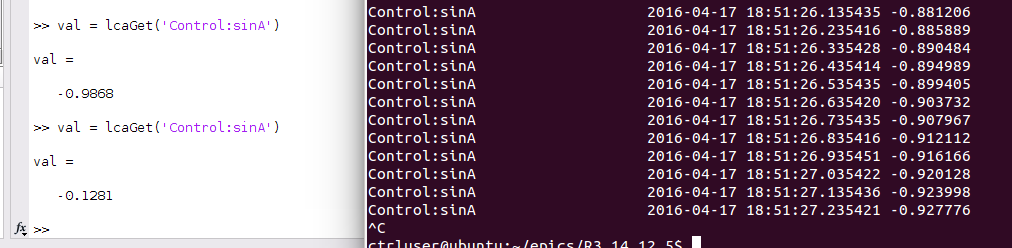
\includegraphics[width=0.85\textwidth]{./images/LabChannelAccess.png}
	\caption{EPICS Matlab Interface}
	\label{fig:lab_channelaccess} 
\end{figure}


\begin{figure}[h!]
	\centering
	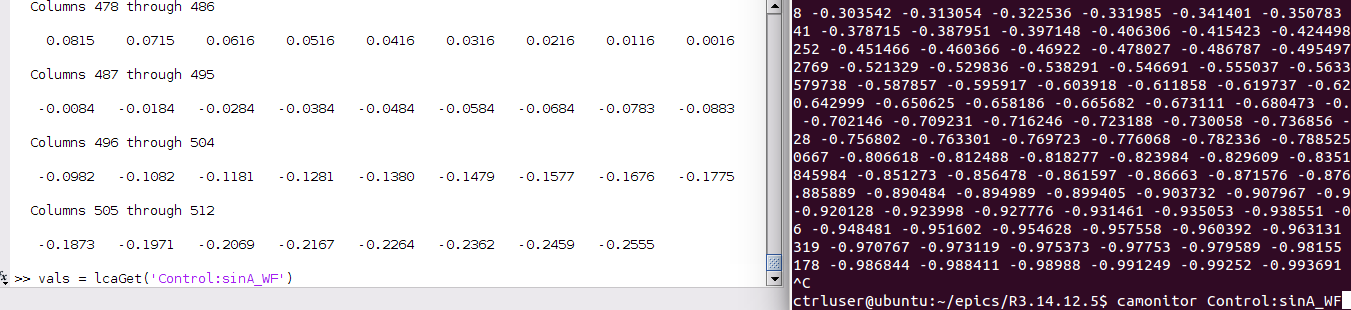
\includegraphics[width=0.85\textwidth]{./images/LabCA_Waveform.png}
	\caption{EPICS Matlab Interface 2}
	\label{fig:lab_channelaccess_2} 
\end{figure}

\clearpage

\clearpage

\bibliographystyle{unsrtnat}
\bibliography{./refs}

\end{document}

